<<<<<<< HEAD

\subsection{Component Integration Sequence}

In this section, it will be described the integration order of the components of the Application Server.
As notation, an arc $C_1 \rightarrow C_2$ means that the component $C_1$ needs the successful integration of component $C_2$.


\paragraph*{Data Access\\}
The first elements to be integrated are \emph{DBMS}, \emph{Account Data Manager} and \emph{Appointment Data Manager}. 
The integration process starts from this point because other components relies on \emph{Account Data Manager} and \emph{Appointment Data Manager} to store data and retrieves data for computation and visualization.
\begin{figure}[H]
	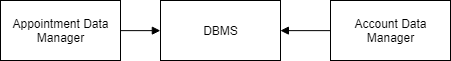
\includegraphics[width=\textwidth, keepaspectratio=true]{Img/FirstStep}
\end{figure}

\paragraph*{Basic Appointment Manager\\}
As second step, \emph{Appointment Data Manager} and \emph{Path Calculator} are integrated in \emph{Appointment Manager}.\\
In this way, it is possible to test how appointments are generated, how are stored and how an appointment interacts with others previous stored appointments.\\
In this step of the integration process, the \emph{Path Calculator} does not consider information about the user preferences, weather conditions or possible strikes, it just provides a path from the departure location to the appointment location.

\begin{figure}[H]
	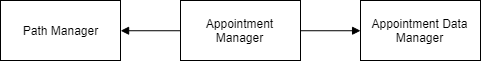
\includegraphics[width=\textwidth, keepaspectratio=true]{Img/SecondStep}
\end{figure}


\paragraph*{Integration of additional info\\}
As third step, \emph{Weather Info Manager}, \emph{Road Info Manager} and \emph{Account Data Manager} are integrated in \emph{Additional Info Façade}.

\begin{figure}[H]
	\centering
	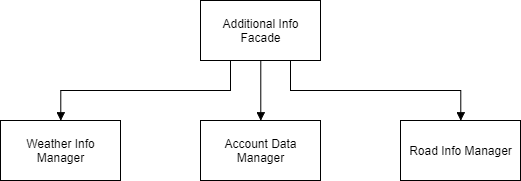
\includegraphics[width=\textwidth, keepaspectratio=true]{Img/ThirdStep}
\end{figure}

\paragraph*{Complete Appointment Manager\\}
As fourth step, the Additional Info Façade is integrated in the Path Calculator component.

\begin{figure}[H]
	\centering
	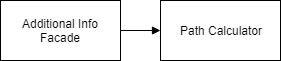
\includegraphics{Img/FourthStep}
\end{figure}

\paragraph*{User Info Management\\}
As final step, it is tested the integration of \emph{Authentication Manager} and \emph{Profile Manager} with \emph{Account Data Manager}.

\begin{figure}[H]
	\centering
	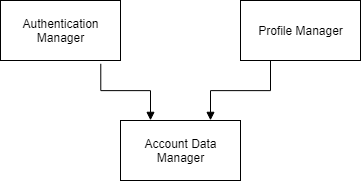
\includegraphics[scale=0.8]{Img/FifthStep}
\end{figure}

\paragraph*{Complete Integration Sequence}
In this diagram is possible to see all the integration steps, numbers on the arrows indicates the precedence, same number on multiple arrows means that is possible to perform the test integration simultaneously.

\begin{figure}[h]
	\centering
	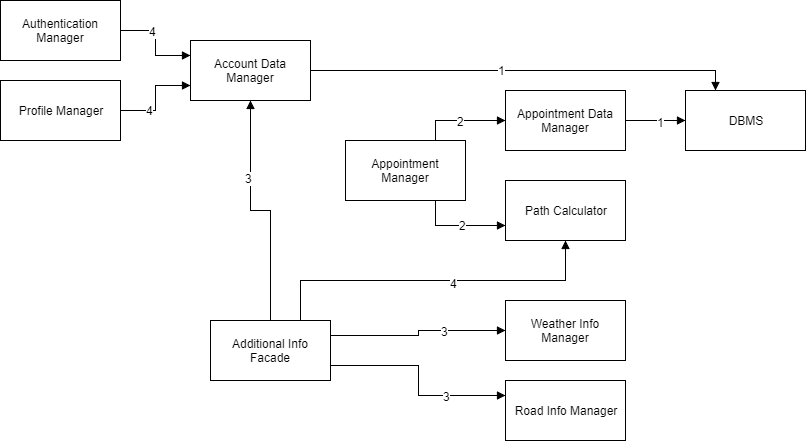
\includegraphics[width=\textwidth, keepaspectratio=true]{Img/IntegrationSequence}
\end{figure}
=======
\subsection{Introduction}
In this section is present the documentation regarding the implementation order of the different components of the system and their integration with one another, also dealing with the test panning for when the code of the system will be written.
\subsection{Entry Criteria}
What follows is an illustration of the requisites that need to be fulfilled before the Integration phase can start.
\paragraph*{RASD \& DD:\\} The RASD and the previous sections of the DD must be completed and delivered before starting to consider the integration or the implementation.
\paragraph*{Unit Testing:\\} Before starting the integration between different components each class and method must be keenly tested using JUnit testing, this is done to ensure that every sub-system is fully functioning on its own, or, in the case that the testing highlights bugs or incorrect behaviour in parts of the code, it allows the team to correct them at an earlier stage, resulting in a lower cost and more time efficient debugging.\\
The JUnit testing should cover no less than the 90\% of the code to be considered satisfactory and each test must be run again at each addition of code and between integrations.
\paragraph*{Documentation:\\} Each method and class must be fully documented using JavaDoc in order to assure that the code is easily understandable, making it easier to extend and maintain even by different people that may end up working on the system in the future.\\
Names of classes, methods and variables must be chosen with the intent of communicating the reason of their existence and not be confusing or too similar to one another, also they should follow the standard Java naming conventions.
\clearpage
\subsection{Elements to be Integrated}
As already stated before, we chose a Four-Tier architecture, so the integration plan will be based heavily on this decision, with the following subsystem to be integrated (this of course means that each one of this subsystem will have to be completely integrated with regard to its internal subsystem too):
\begin{enumerate}[label=\textbf{Tier \arabic*}]
\item \emph{Database}: This tier is composed of the physical database and the DBMS that handles the requests of the higher systems via query to the database itself.\\
It should be noted that the integration of this tier is almost exclusively about the DBMS given that the database should be acquired from dedicated companies as an external system in order to avoid the toll of managing the redundancy and the expansion of the storage modules.
\item \emph{Application Logic}: It includes all the components and subsystems that handle the logic of the system, it should be noted that each individual component should be tested by itself before integrating it with the others and after each integration new tests should be ran to confirm the correct functioning of the integrated subsystems.
\item \emph{Web}: It handles all the interactions between the client's \emph{web browser} and the \emph{web server}, this means managing the interface that will be ultimately be displayed to the user.
\item \emph{Client}: Composed by both the \emph{mobile application} and the \emph{web browser} it's the less logic heavy tier of the system, each client can be seen as a mere presentation system and the integration should focus on making sure that the communication doesn't imply high waiting time and that the graphical interface behaves as it should regarding the received data.
\end{enumerate}
\subsection{Integration Testing Strategy}
As a testing strategy it has been chosen a \textbf{bottom up} approach, the thinking behind this choice can be found by noting that the system is composed by many small components that can be tested individually.\\
This results in a minimal amount of stubs needed during the testing phase (but of course on the other hand there is a need for higher-level modules like drivers).\\
We also decided to integrate elements of a \textbf{critical-module-first} approach in order to give precedence to the core elements (like those containing the application logic) with the intention of conducting a more extensive testing on them and find system-breaking bugs as early as possible given that as it's commonly known it's much easier and cheaper to fix a defective software in the earlier stages of development.\\
Furthermore we note once again that the database is a commercially available solution, while the database management system is an already existing solution that is compatible with the DB, making them ready to use from the start with only the need of configuring the DBMS to communicate with the application server, but it doesn't require any programming in the sense of coding.








>>>>>>> master
